\documentclass[a4paper]{article}

\usepackage[english]{babel}
\usepackage[utf8]{inputenc}
\usepackage{amsmath}
\usepackage{graphicx}
\usepackage[colorinlistoftodos]{todonotes}

\title{Project Specification: Interchangeable Sensors for Modular Camera Systems}

\author{Michael Wild – m.a.wild@se12.qmul.ac.uk \and Supervisor: Miles Hansard – miles.hansard@qmul.ac.uk}

\date{\today}

\begin{document}
\maketitle

\section{Overview}

The aim of this project is to design a sensor-agnostic interface which can be used to connect any image sensor to any processing board, thus providing a truly modular and upgradeable camera system.

Modern cameras (both still-motion and video) have a multitude of upgrade options: lenses, filters and other accessories are all interchangeable, enabling creative freedom and flexibility. As one of the most important components of the system, the photographic sensor plays a vital role in the final image. It dictates not only the output resolution, but also noise, colour response, field-of-view, depth-of-field, frame-rate and cropping. 

In spite of its significance, only a handful of niche cinema cameras include interchangeable sensors; even then, they are only compatible with first-party sensors. Upgrading the sensor in a mainstream camera requires the purchase of an entirely new system.

This project seeks to provide a solid base for continued work on a fully-modular digital camera system with applications in cinema, photography and computer vision.

\section{Methodology}

This project will be conducted in four discrete stages. Initially the focus will be on interfacing with a simple low-resolution sensor module to obtain a single frame of video, providing a solid base for the slave side of the sensor-mainboard link. Next, a connection will be established to transfer image data between the sensor module (slave) and the mainboard (master). Contextual information gleaned from the first stage will be used to design this interface, which should ideally support 1080p resolution images at 24 FPS. Once image data can be transfered successfully, the slave will be replaced with a test pattern generator and tuned to achieve a useful maximum interface bandwidth. To determine the maximum bandwidth, multiple test patterns of increasing resolution / frame-rate / pixel depth will be transmitted through the interface. Bit-error-rate, memory throughput and various other metrics will be used to determine the maximum bandwidth figure. Finally, the image data should be saved to some storage medium (SD card or SSD) for computer analysis / production use.

Once the system successfully works with a simple low-resolution sensor, the system can be modified to support higher-end sensors, time-permitting.

\section{Objectives}

\begin{itemize}
    \item Design prototype camera with simple sensor module
    \item Sensor-agnostic interface and image acquisition pipeline
    \item Support multiple resolutions and frame rates
    \item Test maximum bandwidth with test pattern generator
    \item Storage through either external HDMI recorder or flash
    \item Video playback on host computer
\end{itemize}

\section{Stretch Goals}

\begin{itemize}
    \item Additional high-quality sensor module
    \item Design self-contained enclosure for prototype
    \item Display real-time video monitoring on LCD panel
    \item Overlay video statistics (histogram etc.) on monitor
\end{itemize}

\section{Milestones}

\begin{itemize}
    \item Autumn
    \begin{itemize}
        \item Pick suitable image sensor that supports VGA @ 24 FPS
        \item Choose and acquire appropriate FPGA for interfacing with sensor
        \item Setup and familiarise self with FPGA toolchain
        \item Design and fabricate sensor breakout board if required
        \item Connect and verify sensor and intermediary FPGA
        \item Capture single frame from sensor and output to computer
        \item Plan sensor module interface: data rate, date type, physical requirements etc.
        \item Write interim report
    \end{itemize}
    \item Winter
    \begin{itemize}
        \item Pick appropriate mainboard FPGA / microprocessor combo
        \item Design and fabricate any interposer boards to connect sensor module (sensor + intermediary FPGA) and mainboard (acquisition FPGA + microprocessor)
        \item Write interface blocks for master and slave and clock data into memory
        \item Use test pattern generator to measure maximum interface bandwidth
        \item Build custom Linux kernel for microprocessor
        \item Access framebuffer from Linux and save to storage medium
        \item Write final report and presentation
    \end{itemize}
\end{itemize}

\section{Knowledge Areas}

\begin{itemize}
    \item Existing
    \begin{itemize}
        \item Image Processing
        \item FPGA Design
        \item Embedded Linux
        \item PCB Design
    \end{itemize}
    \item{New}
    \begin{itemize}
        \item High-Speed Interfaces
    \end{itemize}
\end{itemize}

\section{Required Facilities}

EDA software and soldering equipment will be required for the design and manufacture of a custom image sensor PCB and / or interposer boards, as well as test equipment for analysing data buses. Additionally, use of 3D printing / laser cutting will be required in the later stages of the project to produce a protective housing for the sensor and ensure precise lens alignment.

\begin{figure}
\centering
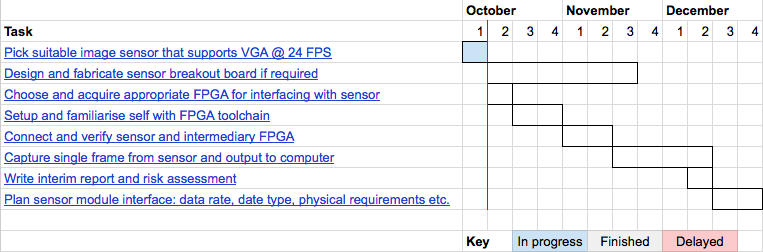
\includegraphics[width=1\textwidth]{gantt_chart.png}
\caption{\label{fig:gantt_chart}High-level GANTT chart for Autumn semester.}
\end{figure}

\end{document}